\documentclass[11pt]{article}
\usepackage[margin=1in]{geometry}
\usepackage{amsmath,amssymb,amsthm}
\usepackage{graphicx}
\usepackage{enumitem}
\usepackage{hyperref}
\hypersetup{hidelinks}

\newtheorem{theorem}{Theorem}
\newtheorem{lemma}{Lemma}
\newtheorem{corollary}{Corollary}
\newcommand{\K}{\mathbb K}
\newcommand{\Qp}{\mathbb Q_p}

\title{A Split Resolution of the Functional Zauner Conjectures:\\
Degenerate Existence and a \(p\)-Adic Impossibility}
\author{Run \texttt{fa\_banach\_001}, agent \texttt{agent\_lane\_05}}
\date{August 11, 2026}

\begin{document}
\maketitle

\section*{Source targets and result}

The source is K. Mahesh Krishna's \emph{Non-Archimedean and p-adic
Functional Welch Bounds}.  It is arXiv:2209.06769 and formulates a
non-Archimedean functional Zauner conjecture (Conjecture 2.5), a \(p\)-adic
functional Zauner conjecture (Conjecture 3.4), two equality questions, and
two functional equiangular-line problems.

This packet proves four exact conclusions.
\begin{enumerate}[label=(\arabic*)]
\item Under the source field axiom, every positive integer has absolute
value one.  On \(\K^d\) with the standard maximum norm, a repeated
vector--functional pair solves Question 2.4 for every \(d\) and \(n\ge2\),
and proves Conjecture 2.5 as literally stated.
\item Conjecture 3.4 is false: for every prime \(p\), no proposed family can
exist in any dimension \(d\) divisible by \(p\).
\item In dimension one, Question 3.3 has a complete answer for \(n\ge2\):
such a family exists exactly when \(p\nmid n\).
\item In both functional equiangular formulations, the parameter choice
\((a,\gamma)=(1,1)\) admits arbitrarily many repetitions.  Hence the stated
problems have no finite Gerzon bound without a distinctness hypothesis.
\end{enumerate}

The decisive source conjectures are reproduced below.
\begin{center}
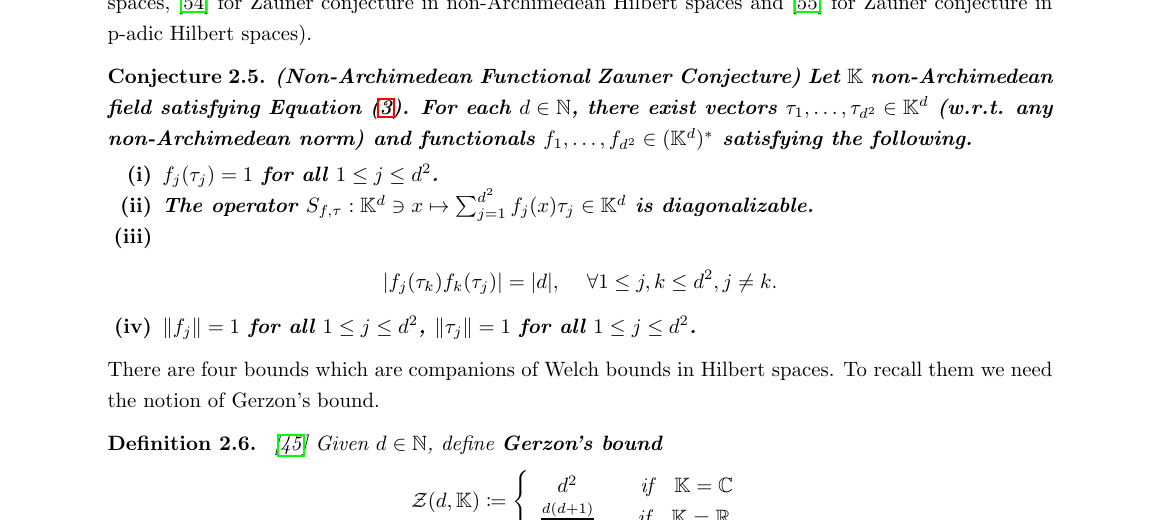
\includegraphics[width=0.94\linewidth]{figures/nonarch_zauner_crop.png}
\end{center}

\begin{center}
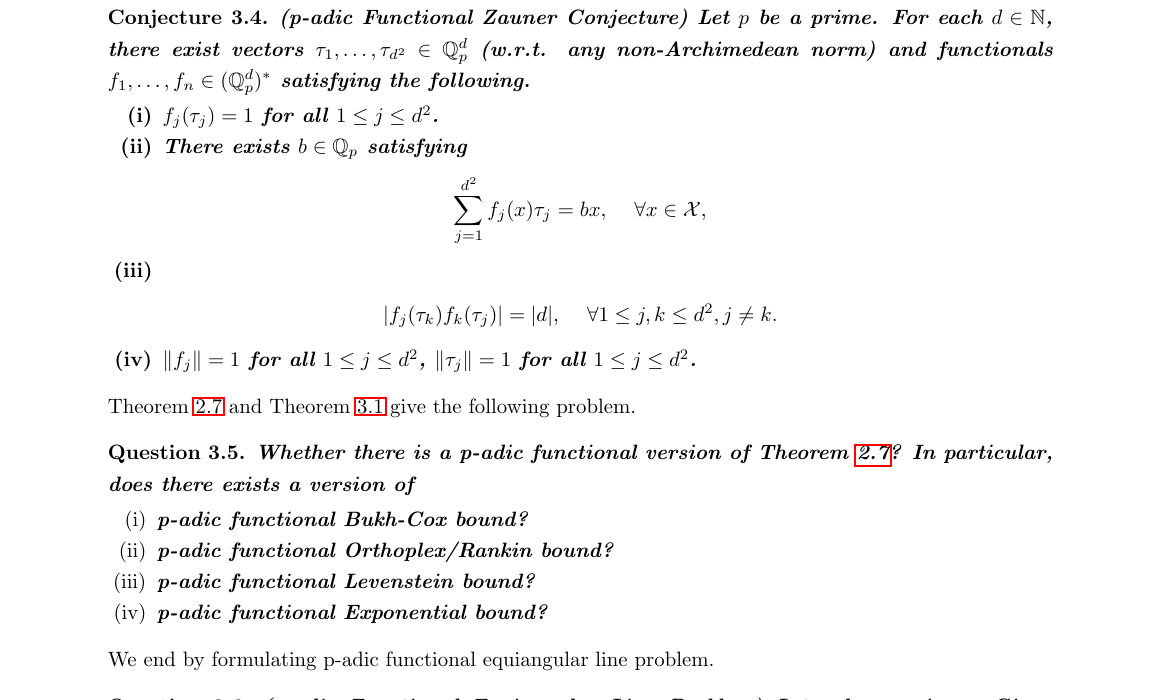
\includegraphics[width=0.94\linewidth]{figures/padic_zauner_crop.png}
\end{center}

\section*{The non-Archimedean functional half}

The source assumes
\begin{equation}\label{eq:FU}
 \left|\sum_{j=1}^r\lambda_j^2\right|
 =\max_{1\leq j\leq r}|\lambda_j|^2
 \quad\text{for every }r\geq1\text{ and }\lambda_j\in\K.
\end{equation}

\begin{lemma}\label{lem:integers}
If \(\K\) satisfies \eqref{eq:FU}, then \(|r|=1\) for every positive
integer \(r\).  In particular, \(\K\) has characteristic zero.
\end{lemma}

\begin{proof}
Take \(\lambda_1=\cdots=\lambda_r=1\) in \eqref{eq:FU}.
\end{proof}

\begin{theorem}\label{thm:nonarch}
Let \(\K\) satisfy \eqref{eq:FU}.  Equip \(\K^d\) with the maximum norm.
For every \(d\geq1\) and \(n\geq2\), all conditions of Question 2.4 hold.
Taking \(n=d^2\) proves Conjecture 2.5 under the same literal reading.
More generally, the construction works in any normed space containing a
norming pair \((u,\varphi)\) with
\(\|u\|=\|\varphi\|=\varphi(u)=1\).
\end{theorem}

\begin{proof}
For the maximum norm take \(u=e_1\) and
\(\varphi(x_1,\ldots,x_d)=x_1\), and repeat
\[
 \tau_j=u,\qquad f_j=\varphi\qquad(1\leq j\leq n).
\]
Then \(f_j(\tau_j)=1\), both norms are one, and
\[
 S_{f,\tau}x=\sum_{j=1}^n\varphi(x)u=n\varphi(x)u.
\]
Since \(P=u\otimes\varphi\) satisfies \(P^2=P\), the operator \(nP\) is
diagonalizable.  For \(j\ne k\),
\(|f_j(\tau_k)f_k(\tau_j)|=1\).  Lemma~\ref{lem:integers} gives
\(|n|=|d|=1\), so Question 2.4's equality reads
\[
 \max\{1,1\}=1=\frac{|n|^2}{|d|}.
\]
For \(n=d^2\), Conjecture 2.5's off-diagonal requirement is
\(1=|d|\), which also holds.
\end{proof}

The phrase ``with respect to any non-Archimedean norm'' is ambiguous.  The
theorem proves existence for the standard norm and for every norm admitting a
norming pair.  It does not invoke a non-Archimedean Hahn--Banach theorem over
an arbitrary nonspherically-complete field.

\section*{The \(p\)-adic conjecture is impossible when \(p\mid d\)}

We read the source's undefined terminal \(n\) in Conjecture 3.4 as \(d^2\),
as required by the displayed vectors, the sum, and conditions (i), (iii), and
(iv).  The contradiction below is independent of all norm choices.

\begin{theorem}\label{thm:padic}
Fix a prime \(p\).  If \(p\mid d\), no vectors and functionals can satisfy
Conjecture 3.4 in \(\Qp^d\).  Consequently the universal \(p\)-adic
functional Zauner conjecture is false.
\end{theorem}

\begin{proof}
Suppose the conjectural family existed, and write
\[
 Sx=\sum_{k=1}^{d^2}f_k(x)\tau_k=bx.
\]
The trace of the rank-one operator \(\tau_k\otimes f_k\) is
\(f_k(\tau_k)=1\).  Taking traces therefore gives
\[
 bd=\operatorname{tr}S=\sum_{k=1}^{d^2}f_k(\tau_k)=d^2,
 \qquad\text{hence }b=d.
\]
Fix \(j\).  Applying \(f_j\) to \(S\tau_j=d\tau_j\) yields
\begin{equation}\label{eq:diag}
 d=1+\sum_{k\ne j}f_k(\tau_j)f_j(\tau_k).
\end{equation}
Every summand on the right after the initial \(1\) has \(p\)-adic absolute
value \(|d|_p\), by condition (iii).  If \(p\mid d\), their sum has absolute
value at most \(|d|_p<1\).  The ultrametric inequality then says that the
right side of \eqref{eq:diag} has absolute value exactly \(1\), while its
left side has absolute value \(|d|_p<1\), a contradiction.
\end{proof}

This also exposes a mismatch in the source's claim that Conjecture 3.4 is a
special case of Question 3.3.  When \(n=d^2\) and \(p\mid d\), the conjecture
sets every off-diagonal product modulus to \(|d|_p\), whereas the equality in
Question 3.3 has right side
\(|d^2|_p^2/|d|_p=|d|_p^3\); these cannot agree.

\section*{Exact one-dimensional \(p\)-adic classification}

\begin{theorem}\label{thm:oned}
For \(d=1\), \(n\geq2\), and the standard norm on \(\Qp\), Question 3.3 has
a solution if and only if \(p\nmid n\).
\end{theorem}

\begin{proof}
In one dimension write \(\tau_j=a_j\) and \(f_j(x)=c_jx\).  The condition
\(f_j(\tau_j)=1\) gives \(c_ja_j=1\), and hence, for every \(j\ne k\),
\[
 f_j(\tau_k)f_k(\tau_j)
 =(c_ja_k)(c_ka_j)=1.
\]
Thus the left side of condition (iii) is \(1\), while its right side is
\(|n|_p^2\).  Equality is possible exactly when \(|n|_p=1\), or
\(p\nmid n\).  Conversely, if \(p\nmid n\), take every \(\tau_j=1\) and
every \(f_j\) equal to the identity functional.  Then
\(Sx=nx\), and all four conditions hold.
\end{proof}

\section*{No finite functional Gerzon bound as stated}

\begin{corollary}
For every \(d\geq1\), both
\(n(\K,1,d,1)\) and \(n(p,1,d,1)\) are unbounded under the source's
displayed definitions (using the standard maximum norm).
\end{corollary}

\begin{proof}
For every prescribed \(N\), repeat \(N\) copies of \(e_1\) and its first
coordinate functional.  Every self-pairing is one, every cross-product is
one in absolute value, and all norms are one.  The source does not require
the vectors, functionals, or represented lines to be distinct.
\end{proof}

\section*{Scope, duplicate boundary, and verification}

This is a full counterexample to the universal \(p\)-adic functional Zauner
conjecture, a full solution of the one-dimensional equality question, and a
literal solution of the non-Archimedean statement for the standard norm.  It
does not construct the four Bukh--Cox/Rankin/Levenstein/exponential analogues,
classify Question 3.3 in higher dimensions, or solve a strengthened
distinct-line problem.

The run contains adjacent packets for arXiv:2210.07062 (the vector, rather
than functional, repeated-vector degeneracy) and arXiv:2209.12833 (a
continuous diagonal-measure obstruction).  Neither contains the trace and
diagonal identity \eqref{eq:diag}, the \(p\mid d\) impossibility, or the
one-dimensional functional classification proved here.  Exact-id and core
keyword searches found no duplicate.  Bounded primary-source web searches
found only the source and its continuous companion, with no later correction
or resolution.

Human review should focus on the natural \(n=d^2\) repair of the source typo,
the trace identity, and the intended force of ``any norm.''  The \(p\)-adic
counterexample itself is norm-independent.

\begin{thebibliography}{9}
\bibitem{source}
K. Mahesh Krishna, \emph{Non-Archimedean and p-adic Functional Welch Bounds},
arXiv:2209.06769 (2022).
\end{thebibliography}

\end{document}
